\chapter{解讀計算結果}\label{ch:results}

計算結束後，可以結合圖形、資料與工作流分析結果。結果圖幫助我們識別趨勢，資料記錄說明圖從哪裡來，儲存的工作流則規定了整個計算條件。本章介紹怎樣閱讀這些材料，並把它們整理成計算報告或研究記錄中能夠解釋清楚的結論。

本章繼續使用氫分子和矽兩組案例。它們分別說明單點能、原子力、結構最佳化、能帶和態密度的閱讀方法。閱讀自己的結果時，也可以依次問三個問題：這次計算是否完成，圖中的量怎樣定義，它能夠支援哪一種結論。

\section{在專案中找到結果}

\subsection{結果儲存在哪裡}

點選左側欄的 \ui{專案瀏覽器}，展開 \ui{Results}，其中的 \ui{Datasets} 儲存資料集，\ui{Plots} 儲存圖形。資料集儲存一次執行產生的計算資訊，圖形以便於閱讀的形式呈現其中一部分。能帶、DOS 和收斂圖都屬於圖形結果，但它們表示的量不同。

雙擊當前版本生成的圖形可以再次檢視。若同一文件已經開啟，應用會轉到該文件。跨版本開啟舊專案時，圖形物件可能無法恢復；可按後文方法用儲存的數值重新繪圖。比較多次計算時，先閱讀圖形名稱和對應的執行記錄，確認當前檢視的是哪一組條件。結果仍然留在專案中，並不表示它自動跟隨最近修改的節點更新。

例如，把 Ecut 從 $20$ 改為 $30$ Ha 後，原先的收斂圖依然表示 $20$ Ha 的那次計算。只有重新執行並生成新的結果，才能比較兩個截斷能。建議在每次試算後立即給圖形寫一個清楚的名稱，避免積累許多難以區分的預設名稱。

\subsection{先讀記錄，再讀圖形}

一張圖可以很快顯示問題，也可能掩蓋條件不一致。閱讀前先確認結構、泛函、贗勢、截斷能和取樣方式，尤其是在專案中同時存在多個結構時。對於最佳化計算，還應區分初始構型和最終構型。

計算報告中不必逐行抄寫日誌，但應保留原始記錄。正式圖注寫出主要條件，附錄或配套檔案儲存完整輸入。這樣既保持正文流暢，也使重要數字能夠被複查。

\section{讀取資料集}\label{sec:read-dataset}

在\ui{Results → Datasets}中選擇一次執行記錄，在資訊瀏覽器核對名稱、時間和說明。資料集標籤通常以\ui{Run}開頭，後接執行時的工作流名稱。多個記錄的顯示名稱相近時，應結合輸入條件辨認，而不只看列表中的先後位置。當前資訊瀏覽器不展開這些計算資料集的全部數值，原始內容需要在完整MATLAB\regmark{}或相應命令工作空間中進一步讀取。

下面列出匯出資料集後常見的資料名稱，幫助把陣列與產生它的任務對應起來。需要讀取原始陣列時，可按下一節將所選資料集匯出到工作空間。

\begin{table}[htbp]
\centering
\caption{常見結果資料名稱的含義。}
\begin{tabularx}{\linewidth}{lX}
\toprule
名稱 & 閱讀時先檢查什麼 \\
\midrule
info & SCF收斂狀態、總能量、能量與誤差迭代歷史；最佳化結束時也可能對應最後一個離子步。 \\
relaxInfo & 幾何最佳化的過程記錄；不要與初始結構的單點info混讀。 \\
symmetry & 原胞和高對稱路徑資訊，用於核對能帶的晶胞與路徑。 \\
bandProcessing & 路徑k點與能帶陣列，橫軸應按相同路徑解釋。 \\
bandProcessing3D & 倒空間平面上的k點、能量及平面名稱。 \\
DOS & 能量取樣及態密度結果，不是某一個原子的投影態密度。 \\
TDDFT & 激發能Et與躍遷向量Z；先核對計算確實完成及其能量單位。 \\
\bottomrule
\end{tabularx}
\end{table}

不是每次執行都有表中所有專案。只做SCF時不應期待出現DOS；只完成對稱性分析時也不會得到電子能量。電子態等資料還可能以物件形式保留，資訊瀏覽器不一定展開其全部細節。日常檢視可使用圖形和日誌，進一步處理原始陣列時可使用完整MATLAB\regmark{}或配套指令碼。

幾何最佳化結果儲存在執行記錄中，Structure分支保留原始模型。要在三維檢視中檢視最終幾何，可按氫分子示例匯入最佳化後的結構檔案，並與最佳化記錄對照。

\subsection{匯出所選專案項到工作空間}

\ui{主頁 → 變數 → 匯出至 MATLAB\regmark{}}把專案瀏覽器當前選中的條目交給相應工作空間。它匯出的是這個專案項物件，不是自動生成一張CSV表；檔案仍應按資料用途另行儲存。變數名由條目顯示名稱形成，空格會去除，不適合作變數名的字元會作調整。

\begin{steps}
\item 在完整MATLAB\regmark{}中使用工具箱時，在專案瀏覽器選擇需要的資料集，先把顯示名稱改為容易識別的\texttt{H2Run}。
\item 選擇\ui{主頁 → 變數 → 匯出至 MATLAB\regmark{}}。
\item 在MATLAB\regmark{}自身的命令視窗用\texttt{whos}核對變數，讀取該專案項的\texttt{data}，再檢視其中的資料名稱。
\item 在讀取陣列前確認單位、結構和維度，按需要寫入MAT檔案或結果表格；最後仍儲存原專案。
\end{steps}

線上版把所選物件放入應用命令視窗的工作空間；這與完整MATLAB\regmark{}的基礎工作空間不同。獨立應用程式可直接檢視結果圖，並透過儲存專案與匯出影象保留結果。

以下程式碼只說明完整MATLAB\regmark{}中已匯出的SCF資料集的讀取方式，變數名應與實際匯出名一致。

\begin{lstlisting}[language=Matlab]
runData = H2Run.data;
keys(runData)
scfInfo = runData('info');
scfInfo.Etot
scfInfo.converge
save('h2-run-data.mat', 'runData');
\end{lstlisting}

若所選的是圖形條目、結構條目或另一種流程的記錄，應先檢視其資料名稱，再選擇對應欄位。


\section{判斷電子計算是否收斂}
\index{Shoulian panduan@收斂判斷}

\subsection{收斂狀態比曲線外觀更直接}

SCF 日誌末尾的收斂資訊說明求解器是否滿足既定條件。能量曲線趨於平坦是有用的現象，卻不能單獨代替收斂判斷。對於一個尺度較大的負總能量，尚未穩定的小變化在圖上也可能幾乎不可見。

本書氫分子參考執行的最後相對密度誤差為約 $8.85\times10^{-9}$，八原子矽晶胞為約 $7.35\times10^{-9}$，兩者均達到該例使用的電子自洽條件。不必要求自己的每一箇中間迭代點與書中完全重合，但應確認最後的狀態與預期一致。

\subsection{怎樣讀雙縱軸收斂圖}

收斂圖的橫軸是電子迭代次數。藍色能量曲線對應左軸的 Energy (Ha)，橙色誤差曲線對應右軸的 Error。兩條曲線使用不同單位和不同刻度，不能根據它們在圖上的交點賦予物理意義。

誤差軸採用對數刻度。若誤差從 $10^{-3}$ 降到 $10^{-6}$，它下降了三個數量級，而不是簡單減少了三個單位。觀察誤差時，先看整體趨勢，再看是否在某個範圍反覆振盪，最後檢視是否達到停止條件。

在氫分子例中，能量較早接近最後的數值，密度仍需繼續收斂。這個現象說明求解的不同指標並不一定同步穩定。若研究目標涉及力或微小的能量差，應使用足夠嚴格的電子精度，而不是在能量圖看起來平滑時手工結束計算。

\subsection{常見的三種收斂形態}

誤差持續下降但達到最大步數時，可以考慮增加允許步數，讓已有的收斂趨勢繼續。若誤差在兩個或多個水平來回擺動，則應先檢查結構、佔據和數值設定。若從開始便出現非有限數值或明顯異常的能量，應回到輸入，檢查原子距離、晶胞和贗勢載入情況。

這幾種情形的處理重點不同。保留一段完整迭代記錄，比只描述“執行失敗”更便於判斷。對照已經成功執行的小例子，也有助於確定問題來自新體系還是通用環境。

\section{比較總能量}
\index{Zong nengliang@總能量}

\subsection{總能量屬於哪一個體系}

總能量依賴原子種類和數量、結構、泛函、贗勢以及數值條件。不同體系的絕對總能量通常不能直接按大小排序。例如，八原子矽晶胞的總能量比氫分子的總能量更負，不能由此推出矽“更穩定”。兩個數字屬於不同的電子和原子體系。

比較晶胞大小不同但組成相同的結果時，可以換算成每原子能量，或按化學式單元歸一化。比較吸附、反應或缺陷時，則需要根據反應式和參考態構造相應的能量差。先寫清比較物件，再做減法，通常比得到一張很長的總能量表更有意義。

\subsection{用氫分子練習能量比較}

在完全相同的盒、泛函、贗勢和截斷能下，氫分子起始構型的總能量約為 $-1.1652136531$ Ha，最佳化後約為 $-1.1659737582$ Ha。後者更低，說明最佳化器在這一模型下找到了較低能的位置。

兩者能量差約為 $-7.60\times10^{-4}$ Ha。這表示從該起點到最佳化結構的能量變化，並不是氫分子從兩個孤立原子形成時的結合能。計算結合能還需要相應的原子參考態，不能把最佳化過程中的能量下降當成化學反應能。

整理結果時，可以列出結構名稱、鍵長、總能量、最終力和收斂狀態。這樣的表格同時保留幾何與電子資訊，比只列出能量更能說明最佳化過程發生了什麼。

\begin{table}[htbp]
\centering
\caption{本書氫分子參考執行的結果}
\begin{tabularx}{\linewidth}{lX}
\toprule
專案 & 參考數值\\
\midrule
初始鍵長 & $1.50000000$ Bohr，約 $0.79376582$ Å\\
初始總能量 & $-1.1652136531$ Ha\\
最佳化後鍵長 & $1.43107436$ Bohr，約 $0.75729194$ Å\\
最佳化後總能量 & $-1.1659737582$ Ha\\
最佳化後力範數 & 約 $5.55\times10^{-5}$ 原子單位\\
計算條件 & PBE，內建 default 贗勢，20 Ha，10 Bohr 立方盒\\
\bottomrule
\end{tabularx}
\end{table}

保留適當的小數位即可。輸入和模型尚未做充分收斂檢查時，列出十幾位小數並不表示這些位數都具有同等物理精度。表中的數值可用於核對隨書示例。

\section{檢查最佳化後的結構}
\index{Yuanzili@原子力}

\subsection{原子力與穩定位置}

原子力表示能量隨原子位置變化的方向和程度。若一個原子沿某一方向受到力，沿合適方向移動通常可以降低能量。對於氫分子，沿鍵方向的力最容易觀察；對稱佈局中，兩個氫原子的力通常具有對應關係。

一個結構能量較低，並不自動意味著每個原子都已處在穩定位置。最佳化結束後，應檢查最後的原子力和最佳化器給出的停止原因。如果只是達到最大步數，結構可能尚未完成最佳化；如果力已經足夠小，則更有理由把它作為當前模型下的平衡構型。

\subsection{檢查最終結構}

把最佳化後的結構開啟後，先檢查原子數量和元素是否不變，再測量需要的鍵長、鍵角或晶格引數。對於分子，整體平移和轉動不改變內部幾何；比較前後座標時，重點應放在相對位置，而不是某個原子的絕對座標是否改變。

本書的Geometry Optimization教程在固定晶胞中最佳化原子位置。若研究晶格常數，需要明確選擇相應的計算方案，例如在多個固定晶格下比較能量，並對每個構型保持適當的內部原子處理。

\subsection{區域性最小值的含義}

最佳化器從給定初始結構出發，尋找附近較低能的位置。對於雙原子分子，這個過程比較直觀；對於複雜分子、表面吸附或缺陷結構，可能存在多個區域性穩定構型。一次最佳化成功並不等於已經遍歷所有可能結構。

可以從幾個有物理意義的起點分別最佳化，再比較最終結構與能量。為每個起點使用清楚的名稱，並保留其來源。這樣，最後挑選較低能構型時，仍能看出它是怎樣得到的。

\section{閱讀能帶圖}
\index{Nengdai@能帶}

\subsection{開啟隨書專案中的能帶結果}

隨書\file{silicon-band-primitive.ks}包含二原子矽原胞、能帶工作流及參考執行的數值記錄。舊專案的圖形條目提示“物件已刪除”時，可用儲存的能帶與DOS陣列恢復圖形。隨書\file{show_reference_results.m}提供相應的重繪命令。

這套重繪步驟在完整MATLAB\regmark{}中使用工具箱的圖形介面，不執行DFT計算。使用獨立應用或線上版時，可按第\ref{ch:workflows}章執行對應工作流，生成當前版本的結果圖。

\begin{steps}
\item 在完整MATLAB\regmark{}中啟動工具箱，從\ui{主頁 → 開啟}讀取\file{silicon-band-primitive.ks}。在\ui{Structure}中核對二位點Si結構，保留這份專案為當前專案。
\item 將MATLAB\regmark{}的當前資料夾切換到本手冊倉庫根目錄，在MATLAB\regmark{}自身的命令視窗執行：
\begin{lstlisting}[language=Matlab]
addpath(fullfile(pwd, 'docs', 'manual-zh-CN', 'examples'));
show_reference_results("bands");
\end{lstlisting}
\item 等待中央出現\ui{EnergyBandStructure}圖形文件，\ui{Results → Plots}也會增加相應條目。先把圖形與\ui{Energy Band}工作流對應起來，確認仍是二原子原胞、每段8點的參考資料。
\item 閱讀橫軸高對稱點標籤和縱軸單位，再用座標區提供的縮放工具檢視零能量附近。需要回到全部能帶時，恢復整體檢視，避免只觀察放大後的一小段。
\item 匯出當前圖片，並將專案另存為自己的副本。以後遇到舊圖形無法恢復時，可再次從儲存數值重繪，不必為恢復一張圖而重新執行電子求解。
\end{steps}

圖\ref{fig:si-band-results}與圖\ref{fig:si-bands-native}顯示同一原胞的參考資料，能帶數值、路徑座標和能量零點一致。圖形文件支援縮放與互動檢視。


\begin{figure}[!htb]
\centering
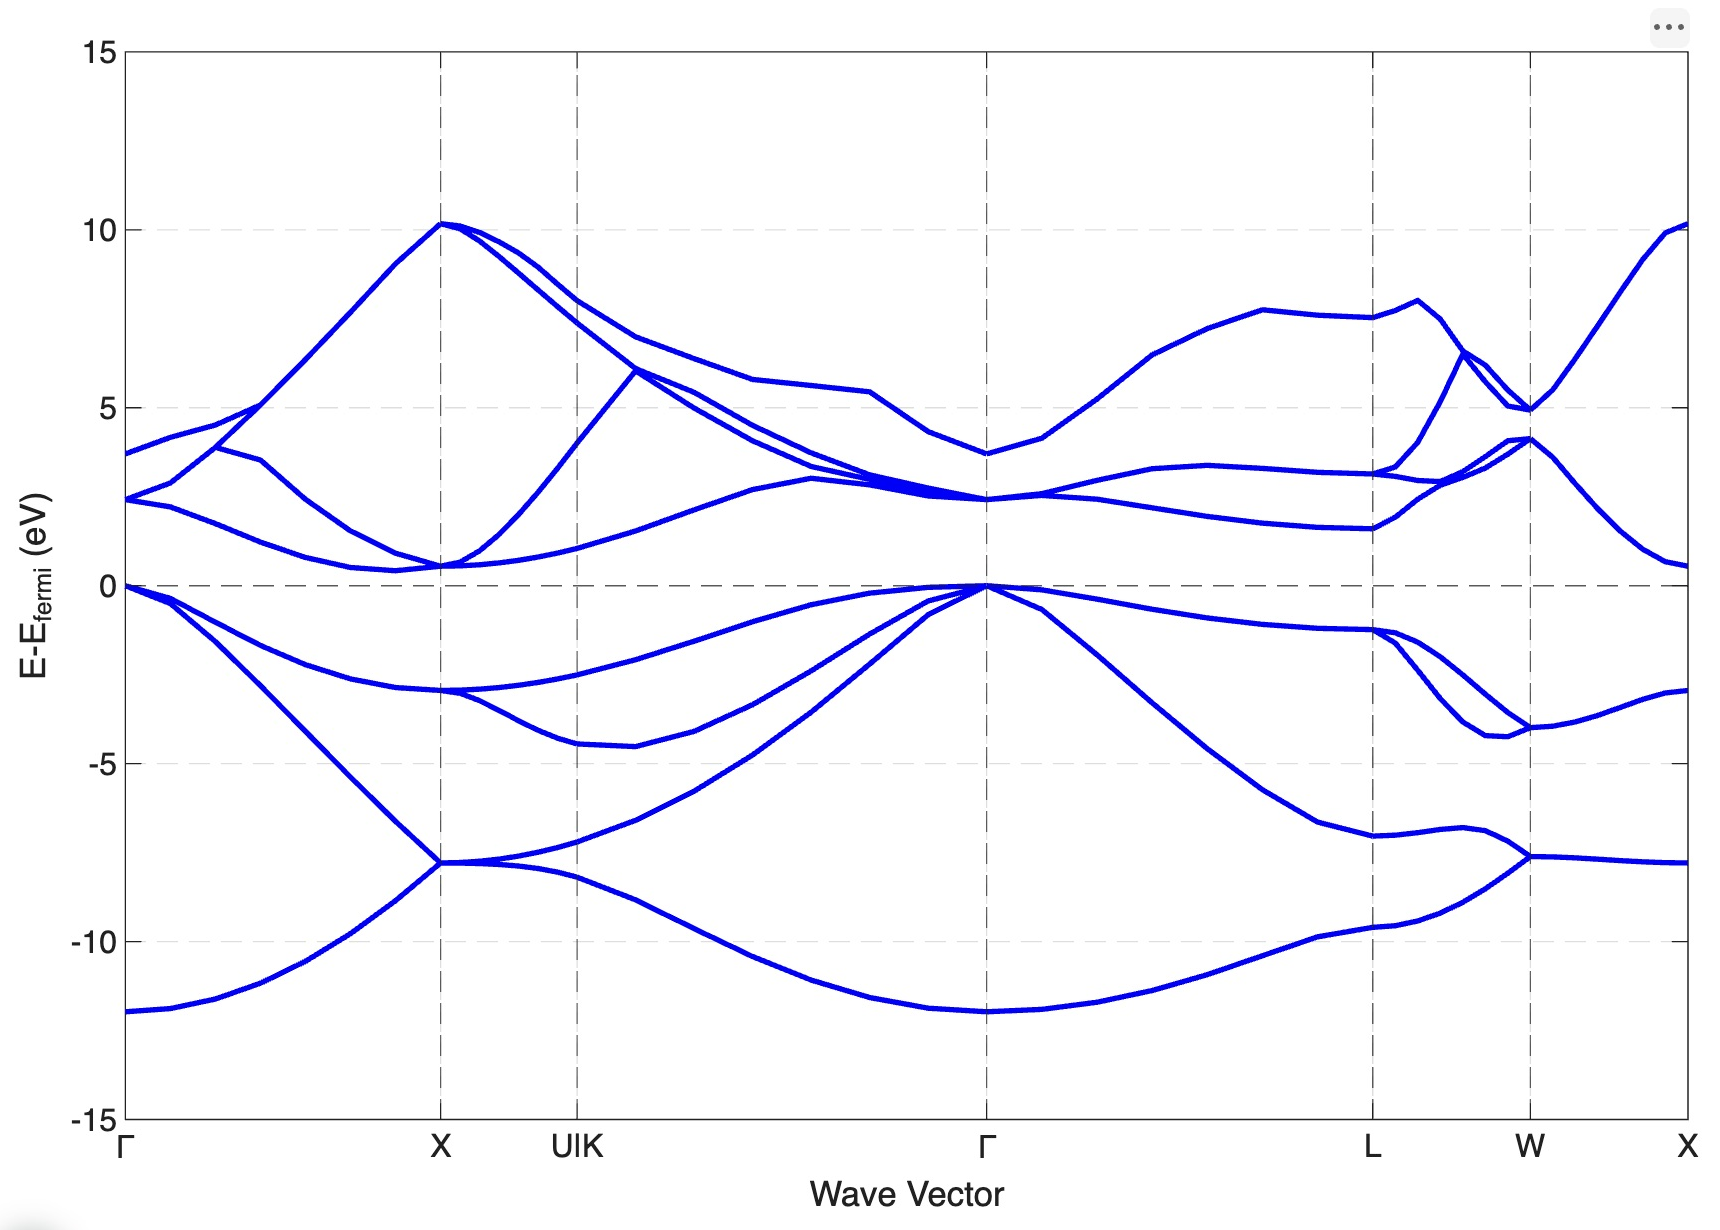
\includegraphics[width=\linewidth]{publication-assets/revision-silicon-bands-live.png}
\caption{矽兩原子原胞的能帶圖形文件。每段路徑取8點，能量以費米能為零點。}
\label{fig:si-bands-native}
\end{figure}

\subsection{先確認座標和零點}

能帶圖橫軸表示一條由若干高對稱點組成的路徑，縱軸表示能量。本書圖中縱軸為 $E-E_{\mathrm{fermi}}$，單位 eV，因此零點是本次計算的費米能參考。不同路徑段之間可能有分隔線或標籤，不一定表示它們在倒空間中都連續相接。

曲線的橫向位置由路徑距離確定，並不是把三個 k 座標中的某一個直接拿來作橫軸。讀圖時可以先辨認路徑標籤，再觀察費米能附近的佔據態與未佔據態，最後檢視更深的價帶或更高的空態。

圖中每一條曲線表示一個能帶分支，不是一個原子的運動軌跡。本例儲存八條能帶，所有曲線採用相同的藍色；不能把線條顏色理解為元素、軌道或自旋分類。沿同一條曲線從左向右閱讀，可以觀察這條帶隨路徑改變的能量；在同一橫座標處由下向上閱讀，則是在比較該k點的不同能帶。

高對稱點之間的豎向虛線用於劃分路徑區段。若兩段並不首尾相接，分界處可以出現組合標籤；例如\ui{U|K}表示前一段到U結束、下一段從K開始，不是名為“U|K”的一個新k點。跨過這種分界時，不應把兩側曲線的接續當作沿同一方向連續行進。

\subsection{判斷帶隙}
\index{Daixi@帶隙}

在通常的半導體描述中，較高的佔據能帶屬於價帶，較低的未佔據能帶屬於導帶。價帶最高點與導帶最低點之間的能量差稱為帶隙。若兩者位於相同 k 點，通常稱為直接帶隙；位於不同 k 點，則稱為間接帶隙。

一條有限路徑不一定經過真正的帶邊位置。即使圖形很平滑，也不能僅憑路徑上沒有出現更低導帶就斷定它已經找到了全布里淵區的最小值。對於帶隙研究，應結合更充分的取樣和帶邊分析。

本書矽例採用較粗的入門網格，便於熟悉計算與繪圖方法；定量帶隙還需要更充分的取樣。整理計算報告時，先說明採用的條件，再討論網格和泛函可能怎樣影響結果。

\subsection{比較兩張能帶圖}

比較之前，檢查晶胞、路徑、能量零點、泛函、贗勢和帶數是否一致。改變原胞與超胞可能導致能帶摺疊，圖上曲線數量增加並不必然表示出現了新的物理態。改變零點也可能使整張圖上下平移。

若研究形變的影響，可以保持同一套計算思路，對各個結構分別完成自洽，再使用可比較的路徑。先觀察變化主要發生在哪些能帶和 k 點，再決定是否需要更精細的取樣。把每一處微小位移都解釋為新的物理效應之前，先排除數值條件不一致。

\section{閱讀總態密度}
\index{Taimidu@態密度（DOS）}

\subsection{開啟並核對總態密度圖}

繼續使用前一節已開啟的\file{silicon-band-primitive.ks}。這份二原子原胞專案同時儲存了一組$4\times4\times4$網格的總態密度數值，可以直接重繪，不必先關閉專案或執行新的DOS流程。

\begin{steps}
\item 確認當前仍為二原子原胞專案。在已經加入隨書示例目錄的MATLAB\regmark{}命令視窗執行：
\begin{lstlisting}[language=Matlab]
show_reference_results("dos");
\end{lstlisting}
\item 等待\ui{Density of States (DOS)}圖形顯示，並在\ui{Results → Plots}中核對新增條目。本圖對應當前專案的Si2原胞，與另一份八原子晶胞專案區分。
\item 先看縱軸\ui{Energy (eV)}，再看橫軸\ui{Density of States (DOS)}。曲線向右伸得越遠，表示相應能量附近的總態密度越高；不能按普通“橫軸能量”的習慣從左向右讀取能區。
\item 沿縱軸找到零能量，再分別檢視其下方、附近和上方的曲線。先描述有態區間、低態密度區間及主要峰，再考慮更細的小起伏。
\item 使用圖形儲存工具匯出當前曲線，並保留含原始結果的專案。重新開啟圖片檢查兩個座標軸都在畫面中。
\end{steps}

這組DOS在$-10$至$10$ eV之間以$0.05$ eV步長取樣，使用PBE、default贗勢和20 Ha截斷能。希望改變網格或能量範圍時，按第\ref{ch:workflows}章匯入\ui{DOS}模板，選擇二原子原胞，填寫新的引數並執行；重繪已有陣列本身不會增加取樣精度。




\begin{figure}[!htb]
\centering
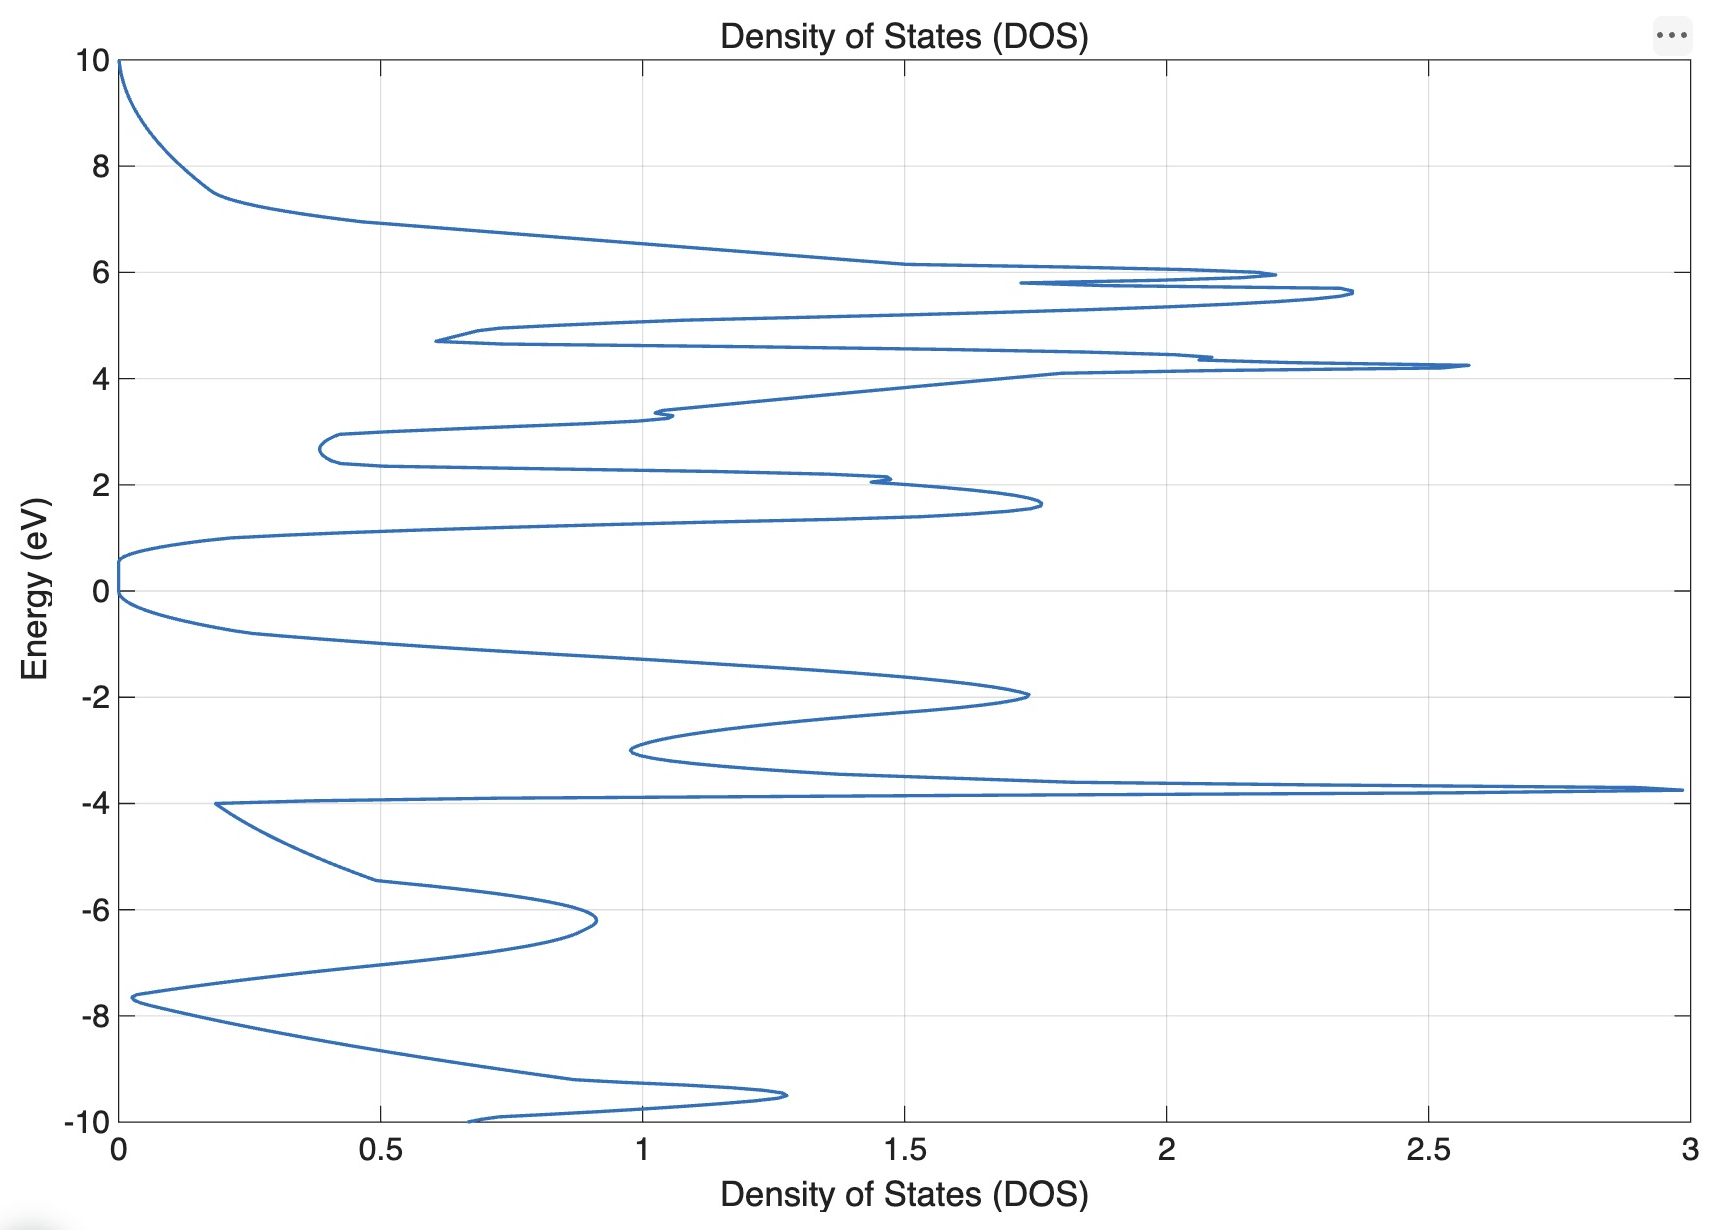
\includegraphics[width=\linewidth]{publication-assets/revision-silicon-dos-live.png}
\caption{同一矽兩原子原胞的總態密度圖，橫軸為態密度、縱軸為相對費米能的能量。}
\label{fig:si-dos-native}
\end{figure}

\subsection{峰和低密度區域}

態密度在某個能量附近較高，表示這一能量範圍聚集了較多電子態。曲線中的峰往往與能帶的色散特徵有關，但峰本身不直接告訴我們電子主要來自哪一種原子或軌道。那需要進一步的投影或成分分析。

DOS節點給出總態密度，彙集了不同軌道和k點的資訊。判斷某個峰的元素或軌道成分，需要相應的投影態密度資料。

\subsection{與能帶圖聯合閱讀}

把能帶和 DOS 放在相同能量參照下，可以先定位費米能，再觀察哪些能區有較多電子態，哪些能區沒有態。能帶圖展示沿路徑的變化，DOS 則彙總整個網格的統計，兩者從不同角度描述同一電子結構。

\file{silicon-tutorial.ks}另存八原子常規晶胞的DOS數值。開啟那份專案再執行同一條\texttt{show\_reference\_results("dos")}命令，得到的是Si8結果。下文圖\ref{fig:si-dos-results}保留這份八原子參考曲線，供閱讀座標與峰形；它與前述原胞重繪對應不同晶胞。比較兩者時，先統一每晶胞或每原子的歸一化方式，以及計算條件和能量參照。

\begin{figure}[!htb]
\centering
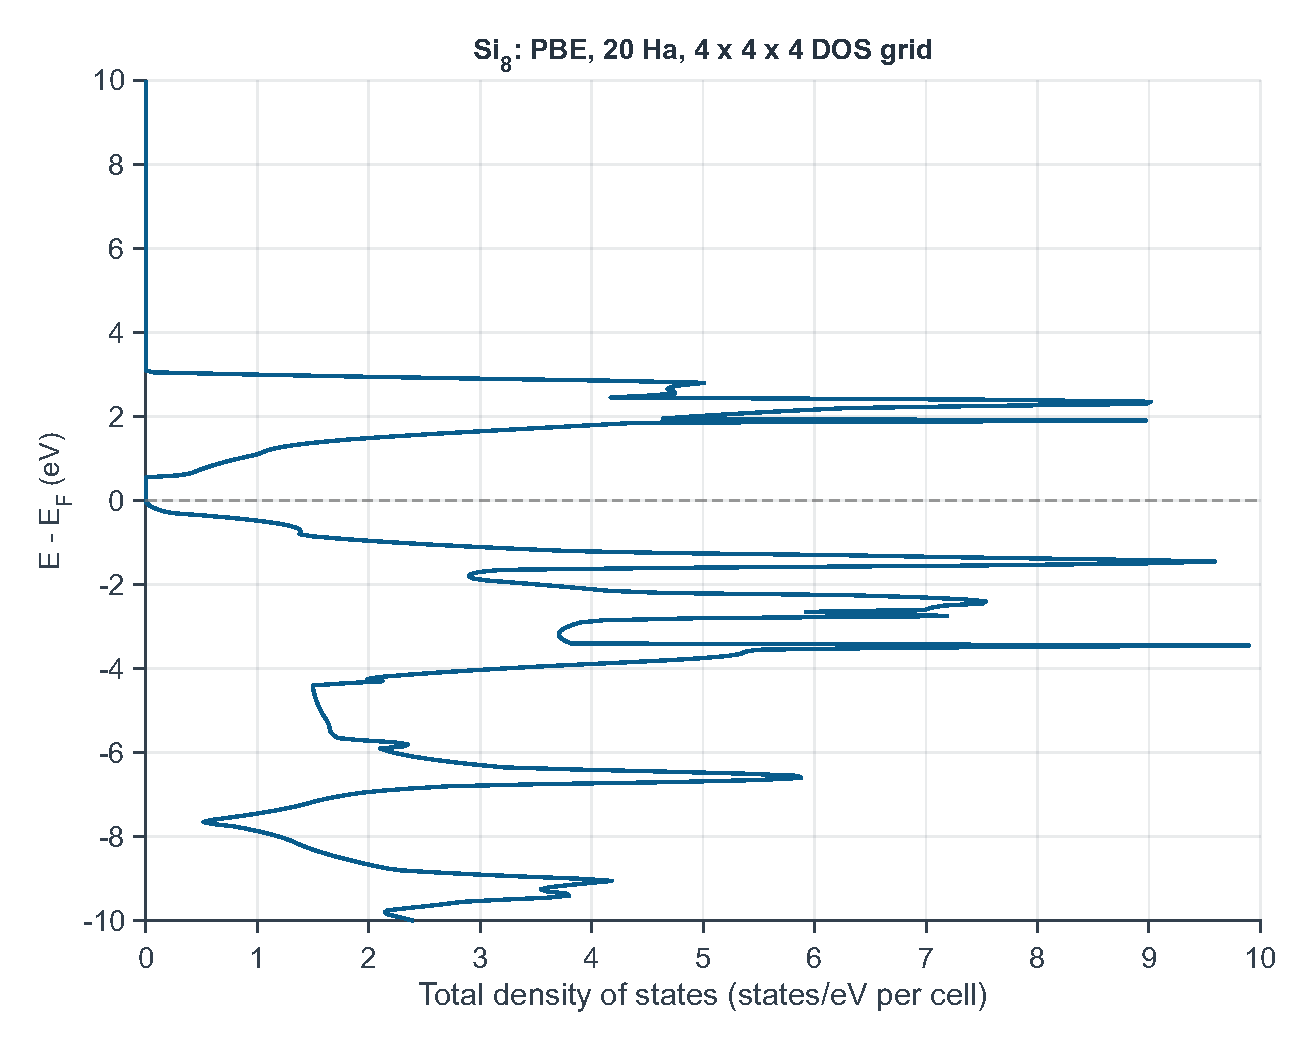
\includegraphics[width=\linewidth]{publication-assets/vector-02b7a0240bc7f99a0fc6.pdf}
\caption{八原子矽晶胞的參考總態密度。橫軸為每晶胞、每電子伏特的態數，縱軸為相對費米能；本圖採用入門練習的 $4\times4\times4$ 網格。}
\label{fig:si-dos-results}
\end{figure}

本軟體的 DOS 圖橫軸為 DOS，縱軸為 Energy (eV)。若報告中把 DOS 放在能帶圖右側，這種排列能夠讓兩幅圖共享由下到上的能量閱讀方向。最終排版時，應保持兩圖的能量範圍和零點一致。

\subsection{分辨取樣細節與物理特徵}

粗 k 點網格可能使 DOS 峰形變化明顯，特別是在電子態較少或色散較強的能區。減小能量步長只能更密地評價當前近似曲線，不會增加布裡淵區中的資訊。判斷某個小峰是否可靠，應比較更密網格下它是否仍然存在。

本書 $4\times4\times4$ 的矽 DOS 是入門起點。若把網格提高到 $8\times8\times8$，應比較主要峰位、費米附近低態密度區域和整體形狀，而不是隻看圖線是否變得好看。不同精度下穩定保留的特徵更值得繼續分析。

\section{核對三維結果}

幾何圖適合展示原子位置、晶胞和區域性環境。電子密度、勢或軌道等空間資料則需要體資料檢視器。匯入實際的體資料檔案後，可以使用等值面、切片和顏色對映觀察它們的空間分佈。

體資料的含義由輸入檔案和資料型別決定。一個標註為電子密度的 CUBE 檔案與一個標註為軌道幅值的 CUBE 檔案，雖然都能形成等值面，顏色和數值的物理解釋卻不同。先確認變數和單位，再選擇等值面數值。

展示電子密度、勢或軌道等空間量時，先準備相應的體資料檔案，再按第\ref{ch:volume}章匯入。圖注中註明變數、等值面值和單位。

\section{整理原子結構檢視}

本節使用原子結構文件自己的檢視器。先開啟隨書矽結構，或開啟已經檢查過連線的分子，再從檢視工具欄進入\ui{Viewer settings}。這裡的設定用於觀察和製圖；工作流中的泛函、截斷能和電子取樣仍在計算節點中配置。

\subsection{記錄位點與晶胞讀數}

單擊一個原子，在資訊卡中核對位點序號和週期映像，再使用笛卡爾座標或分數座標旁的複製按鈕，將數值貼上到實驗記錄。複製保留的精度高於面板簡寫；笛卡爾座標帶\AA，分數座標沒有長度單位。記錄週期映像時，同時寫出\ui{Image}偏移，避免把相鄰晶胞的顯示位置當作輸入位點的位置。

需要檢視整張座標表時，單擊檢視工具欄的\ui{Structure information}資訊按鈕，其提示為\ui{Fractional coordinates}。表中列出ID、元素、標籤和五位小數的分數座標，適合按位點查詢；需要保留完整數值仍匯出原生結構。分子沒有周期分數座標時，相應列顯示橫線。

晶體的胞長、夾角和體積可以從測量選單的\ui{Cell parameters}讀取。使用讀數旁的複製按鈕，將所需一組值貼上到記錄中，再補上結構檔名和當前晶胞表示。完成後關閉資訊面板，繼續取景；複製讀數不會把模型另存為結構檔案。

\subsection{比較晶胞表示和成鍵策略}

\ui{Scientific scene}集中管理場景分析。晶體的\ui{Change unit cell}可選\ui{Input cell}、\ui{Primitive cell}、\ui{Conventional cell}，以及Niggli和LLL兩種約化晶胞。它們改變當前場景採用的晶胞表示；要把轉換提交為專案中的模型，仍按建模章節使用原胞、慣用胞等結構命令。\ui{Repeat cell}則控制顯示重複範圍，不能代替構建計算超胞。

\begin{steps}
\item 開啟矽結構的檢視器設定，在\ui{Scientific scene}中保持\ui{Input cell}，記下當前位點數和晶胞。
\item 將\ui{Change unit cell}切換為\ui{Primitive cell}，等待場景重建完成。比較晶胞外框與位點排列，再切回\ui{Input cell}，確認回到原輸入的表示。
\item 在\ui{Bonding strategy}中比較\ui{CrystalNN}與\ui{Minimum distance}，觀察顯示連線是否變化。一次只改一項，等待分析完成再讀配位數或最近鄰。
\item 將\ui{Repeat cell}的一個方向設為2，檢查週期接續；完成後用\ui{Reset to 1 × 1 × 1}恢復。記錄用於最終圖片的表示、成鍵策略和重複範圍。
\end{steps}

\begin{table}[htbp]
\centering\small
\caption{晶體檢視器中的成鍵策略。}
\begin{tabularx}{\linewidth}{lX}
\toprule
選項 & 用途與讀數的含義 \\
\midrule
CrystalNN & 按區域性環境分析近鄰，適合從完整配位環境開始觀察。\\
Custom bonds & 使用VESTA截斷規則；這裡選擇規則，不是在此輸入任意鍵長。\\
Jmol bonding & 使用Jmol成鍵判據，便於與相應表示比較。\\
Minimum distance & 以最近距離及介面標出的10\%容差判斷近鄰。\\
O'Keeffe's algorithm & 按O'Keeffe判據識別近鄰。\\
Hoppe's ECoN algorithm & 按有效配位分析識別近鄰。\\
Brunner's reciprocal & 使用Brunner倒數距離判據。\\
\bottomrule
\end{tabularx}
\end{table}

分子的選項不同：\ui{Source topology · preferred}優先使用源連線，\ui{Source topology · explicit}明確使用源拓撲，\ui{OpenBabelNN · inferred}按幾何推斷。已有顯式鍵的苯、吡啶或聚合物應先檢查源連線，再決定是否比較推斷結果。改變顯示連線不會自動完成化學鍵編輯；需要改變分子拓撲時，使用新增鍵、刪除鍵或設定鍵級。

\begin{figure}[H]
\centering
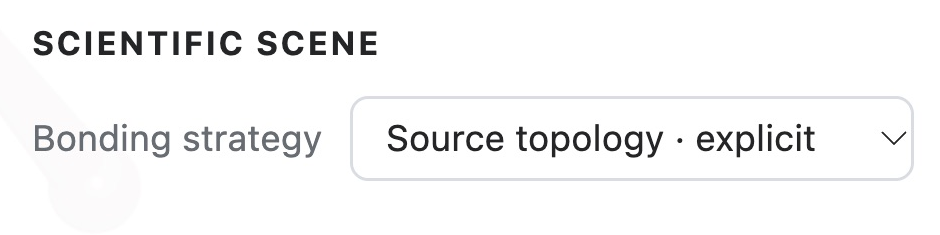
\includegraphics[width=90mm]{publication-assets/crop-1dadf5469e77f06dffe5.png}
\caption{中性單重態乙醇的\ui{Scientific scene}區域性。該輸入有9個原子、8條顯式鍵，當前選擇\ui{Source topology · explicit}，按原始連線顯示分子。}
\label{fig:atomic-scientific-scene}
\end{figure}

\subsection{控制週期邊界和輔助物件}

在\ui{Visibility}中先保留\ui{Atoms}、\ui{Bonds}和晶體的\ui{Unit cell}。\ui{Boundary image atoms}控制邊界映像，\ui{One-hop bonded atoms}補充與當前顯示原子直接相連的一層近鄰，\ui{Hide incomplete bonds}隱藏缺少完整端點的連線。這幾項會改變邊界外觀，應結合位點與映像編號閱讀，不能只數畫面中的球。

需要看區域性配位時開啟\ui{Polyhedra}；需要標明方向時保留\ui{Orientation axes}。\ui{Magnetic moments}用於顯示資料中已有的磁矩，不會計算磁矩。分子另有\ui{Hydrogens}和\ui{Multiple bond order}，分別控制氫與多重鍵的顯示。\ui{Continuous measurement}決定一次測量完成後是否繼續選取下一組；連續測量不改變原子座標。

在\ui{Style}中比較VESTA與Jmol元素配色，按圖的用途選擇\ui{Atomic}或\ui{Uniform}半徑，再調整\ui{Atom scale}和\ui{Bond radius}。原子比例過大時可先減小球體，再判斷是否有真正的短接觸。\ui{Lighting \& surface}中的光照、材質、亮度和對比度用於改善辨識；需要回到起點時使用\ui{Reset appearance}。為一組比較圖採用相同外觀，並另外記錄決定科學含義的結構和測量條件。

\section{匯出原子結構檢視}
\index{Yuanzi jiegou tuxiang@原子結構影象}

原子檢視器的\ui{Export image}輸出當前三維結構圖，\ui{Export file}輸出可互動頁面、場景或結構檔案。它們與體資料的等值面匯出、工作流圖形的儲存工具分別工作。匯出前先停止自動旋轉、清除無關選擇並確定取景。

\subsection{選擇六種影象格式}

\begin{table}[H]
\centering\small
\caption{原子結構檢視器的影象匯出選項。}
\begin{tabularx}{\linewidth}{lX}
\toprule
選單選項 & 適合的用途 \\
\midrule
PNG & 無損點陣圖，適合技術文件與螢幕閱讀。\\
JPEG & 壓縮點陣圖，便於分享；細線和文字應檢查壓縮效果。\\
TIFF & 無損點陣圖，輸出副檔名為\file{.tif}。\\
SVG & 向量表達，適合繼續排版或編輯線條。\\
PDF (Vector) & 向量PDF，便於排版與放大閱讀。\\
PDF (Raster) & 以柵格渲染保留當前場景的顯示效果。\\
\bottomrule
\end{tabularx}
\end{table}

\begin{steps}
\item 開啟需要的結構，調整視角和表示方式，確認晶胞、原子與必要標註都在畫面內。
\item 在結構檢視工具欄開啟\ui{Export image}，先選PNG，填寫儲存位置；線上版完成瀏覽器下載。
\item 需要向量版本時再匯出SVG或\ui{PDF (Vector)}。向量表達與柵格光照可能存在外觀差別，應開啟實際檔案比較後選擇。
\item 檢查匯出圖的邊界、文字和區域性連線，把它與原始結構、專案及本次取景說明儲存在同一練習目錄。
\end{steps}

本選單不使用後文計算結果圖的72至600DPI設定。影象檔案儲存檢視，不能據它重新取得完整的結構座標；交換模型時還應匯出結構檔案。

\begin{figure}[H]
\centering
\begin{minipage}[t]{58mm}
\vspace{0pt}
\centering
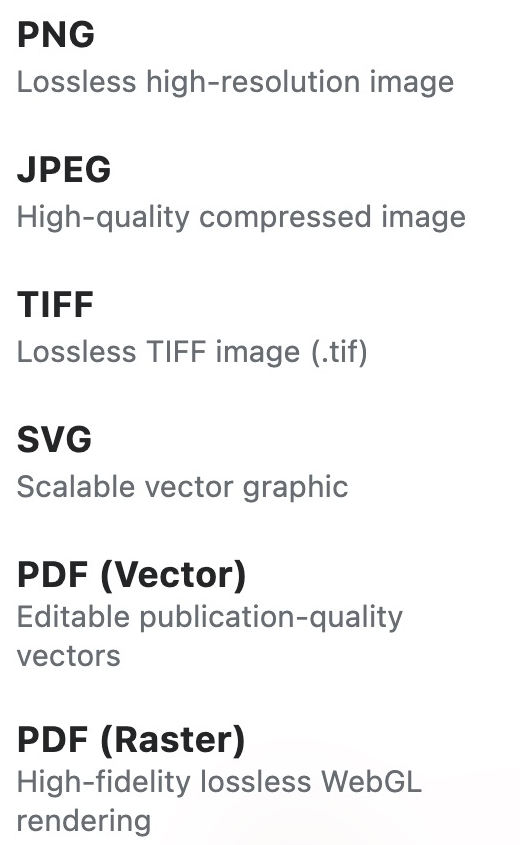
\includegraphics[width=52mm]{publication-assets/crop-496bc1fbfb3e99bfc4e7.png}
\end{minipage}\hspace{4mm}%
\begin{minipage}[t]{58mm}
\vspace{0pt}
{\centering
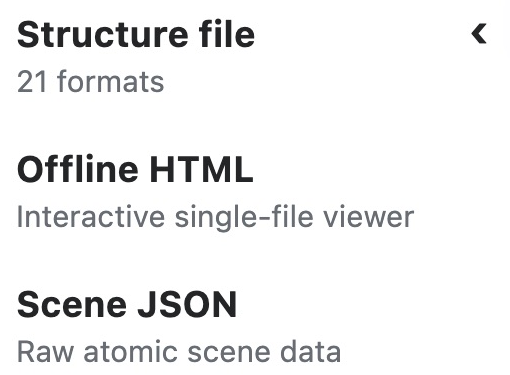
\includegraphics[width=51mm]{publication-assets/crop-68b4df9ea7d48ce9da1e.png}\par}
\par\vspace{3mm}
\raggedright\fontsize{9}{13}\selectfont
\ui{Structure file}儲存所選格式能表達的模型資訊。

\smallskip
\ui{Offline HTML}用於在本機瀏覽器中旋轉觀察。

\smallskip
\ui{Scene JSON}記錄原子場景，區別於結構JSON。
\end{minipage}
\caption{原子檢視器的兩類匯出選單。左側\ui{Export image}提供六種影象格式；右側\ui{Export file}分別通向結構檔案、離線頁面與場景JSON。}
\label{fig:atomic-export-menus}
\end{figure}


\subsection{儲存可以離線旋轉的頁面}
\index{Lixian HTML@離線 HTML}

\ui{Offline HTML}把當前原子場景、檢視器外觀設定與相機一起放入一個HTML檔案，適合隨計算報告提供可旋轉的結構。它用於閱讀場景，不能代替包含工作流、計算資料和編輯過程的專案。

\begin{steps}
\item 在原子結構檢視中選好表示、重複範圍和初始視角。
\item 開啟\ui{Export file}，選擇\ui{Offline HTML}，儲存或下載生成的\file{-offline.html}檔案。
\item 在本機瀏覽器中開啟該檔案，檢查初始結構與外觀，拖動旋轉、滾輪縮放，並檢視所需原子資訊。
\item 分享時同時給出檔案所表示的結構名稱和用途；若還需繼續建模或計算，再附原生結構與專案檔案。
\end{steps}

離線頁面保留匯出時的場景。需要由工具箱重新分析成鍵、轉換晶胞或繼續提交模型時，回到原專案操作，再匯出新的頁面。

\subsection{區分場景\headinglatin{JSON}與結構\headinglatin{JSON}}

同一\ui{Export file}選單中的\ui{Scene JSON}儲存當前原子場景資料，可用於檢查場景中的位點、顯示映像、連線及分析說明。它沒有把當前相機和全部外觀設定一起寫成檢視器配置，也不是匯出專案或計算輸入的替代方式。

繼續編輯模型時，在\ui{Structure file}子選單中選擇原生JSON。重新匯入後可檢視晶格、位點、週期與屬性，其中\file{properties}可保留扭轉角、SQS搜尋記錄等資訊。名稱帶\file{-scene.json}的檔案用於場景記錄；\ui{Offline HTML}用於離線閱讀。按用途命名可便於區分。

隨書的\file{ethanol-angle1095.json}是本節使用的中性單重態乙醇，包含9個原子、8條顯式鍵，按1(C)—2(C)—3(O)定義的鍵角為$109.5^\circ$。\mbox{\file{ethanol-angle1095.png}}是同一模型透過PNG選單匯出的4032\,$\times$\,1964畫素影象；\file{ethanol-angle1095-scene.json}則儲存原子場景。繼續編輯時匯入結構JSON，後兩份分別用於插圖與檢查場景記錄。

\subsection{製作\headinglatin{Hero Shot}展示圖}
\index{Hero Shot@Hero Shot}

Hero Shot提供另一種原子場景展示方式，適合突出整體形態和空間層次。它透過逐步細化渲染生成PNG，所用光照和材質不改變模型位置或電子結構結果。

\begin{steps}
\item 在結構檢視器設定的\ui{Style → Theme}中選擇\ui{Gleamoe Noir}。
\item 向下找到\ui{Hero Shot}，單擊\ui{Enter Hero mode}。設定面板收起，進入專用取景介面。
\item 旋轉、縮放結構，必要時用晶軸按鈕確定方向。構圖後保持檢視穩定，讓漸進渲染細化。
\item 開啟\ui{Export Hero Shot}，先選\ui{High}。\ui{High}、\ui{Ultra}、\ui{Poster}分別標為視口的2.5、3和4倍匯出比例。
\item 選擇儲存位置，等待渲染和寫入結束。開啟生成的\file{-hero.png}檢查邊界與細節；線上版還需確認瀏覽器下載完成。
\item 單擊\ui{Exit Hero mode}返回普通檢視器，繼續測量或編輯；專案和原生模型仍按各自的儲存步驟保留。
\end{steps}

首次練習用小模型與High設定，更容易比較取景和渲染效果。普通結構圖適合清楚標註和幾何比較；Hero Shot適合呈現形態，科學說明仍應給出模型來源、週期及必要的尺寸。

\section{匯出計算結果圖}

\subsection{選擇適合用途的格式}

圖形文件提供座標軸工具，可以縮放、平移並匯出影象。匯出前先調整檢視，確認標籤完整、單位可見、線條沒有被裁切。截圖適合記錄介面操作，正式報告中的資料圖則通常更適合直接匯出。

PNG 等點陣圖格式適合放入文件和演示。PDF、SVG 等格式適合保留線條與文字的清晰度，但複雜圖形或某些渲染內容可能採用不同輸出方式。匯出後開啟檔案，檢查文字、線條和渲染效果。

在線上版中，匯出檔案透過瀏覽器下載。下載完成後，請到瀏覽器實際使用的下載位置檢查檔案；伺服器端的會話路徑不同於個人計算機上的儲存位置。桌面版則根據檔案對話方塊選擇位置。

\subsection{在圖形中檢視細節}

把滑鼠移到圖形座標區，按當前圖形提供的工具進行平移、縮放、旋轉或恢復檢視。二維收斂圖適合放大最後幾步；布里淵區和能帶曲面適合旋轉。檢視區域性後先恢復整體範圍，再匯出需要完整呈現的結果，避免只儲存一段被偶然放大的曲線。

三維能帶曲面主要顯示兩張帶邊曲面。曲面之間的間隔不能未經座標和取樣檢查就當作材料全域性帶隙；沿另一個方向可能還有更低的導帶底或更高的價帶頂。布里淵區圖顯示的是倒空間幾何，也沒有由多面體顏色編碼出電子能量。能帶曲面、布里淵區、路徑能帶與DOS分別表示不同的量，圖注中應寫明圖形型別。

\subsection{在線上版中匯出結果圖}

線上版保留圖形原生工具條，但儲存和複製動作透過瀏覽器取得檔案。選擇儲存影象後，會出現\ui{匯出圖片}視窗，可填寫檔名、格式和解析度。專案儲存與圖片下載分別進行。

\begin{steps}
\item 開啟需要的結果圖，把座標範圍恢復到希望儲存的狀態。
\item 從圖形工具條選擇儲存，填寫有辨識度的檔名，例如\file{H2-SCF.png}。
\item 按用途選PNG、JPEG、TIFF、PDF或SVG。點陣圖解析度可在72至600DPI之間設定；螢幕閱讀可先使用150DPI，列印用途再提高。
\item 單擊\ui{儲存}，隨後完成瀏覽器的檔案下載動作。
\item 從本機檔案管理器開啟實際下載檔案，確認座標軸、圖例和圖注需要的數值清楚完整。
\end{steps}

複製影象與複製向量在瀏覽器環境中也會轉為相應內容的檔案取得流程；向量動作提供SVG來源，不保證直接進入本機系統剪貼簿。選擇PDF或SVG時，DPI不能替代對字型、線條和實際輸出效果的檢查。儲存影象也不會儲存全部原始陣列，所以還應保留專案和必要的資料檔案。


\subsection{儲存原始數值}
\index{Shuju daochu@資料匯出}

專案檔案儲存執行資料，配套指令碼還提供 MAT 或 CSV 結果，適合進一步計算和繪製統一樣式的圖。CSV 表格應有清楚的列含義，例如第一列為相對費米能的能量，第二列為 DOS。交換資料時，另附一行單位說明往往比依賴口頭解釋可靠。

需要擬合、積分或數值比較時，使用原始計算記錄。截圖適合展示趨勢，讀出的點會受到顯示範圍、解析度和線寬影響。

\subsection{一幅可以獨立閱讀的圖}

好的圖注應讓讀者在不翻閱整個專案的情況下理解圖形。結構圖說明原子或晶胞，收斂圖說明迭代量和單位，能帶圖說明路徑與能量零點，DOS 圖說明取樣和能量參照。主要計算條件放在圖注或附近正文即可，不需要把完整日誌擠進圖內。

為多張圖使用一致的字型、字號、顏色和能量範圍。不同圖如果使用同一種顏色表示同一種量，讀者便更容易比較。氫分子的初始與最佳化結構可以使用相同視角；兩個 DOS 可以保持相同軸限；這些安排比增加裝飾更能提高可讀性。

\section{把結果寫成一段完整說明}

一段清楚的結果說明通常依次交代問題、條件、觀察和解釋。例如，可以先說“在固定 $10$ Bohr 模擬盒中最佳化氫分子的鍵長”，隨後給出 PBE、贗勢和截斷能，再報告鍵長縮短與能量降低，最後說明這些數值屬於當前模型下的平衡結構。

避免只寫“結果正常”或“符合預期”。更有用的表達是指出哪個量收斂、主要變化發生在哪裡、比較時保持了哪些條件。數值精度則結合截斷能、取樣和收斂條件說明。

在關閉專案之前，儲存當前工作，重新檢查一次專案、輸入檔案和匯出圖形是否對應。一個能夠開啟、閱讀和再次執行的專案，是這次計算最完整的記錄。
